\chapter{The GARCH Family}
\label{ch:garch}

\begin{application}[Why This Chapter?]
GARCH models forecast volatility using only daily returns, without intraday data.
Project~1 (HARQ-X) uses GARCH as a comparison baseline, and Realized GARCH and the
HEAVY model bridge the daily-return and realized-volatility worlds.
\end{application}

Chapters~\ref{ch:rv}--\ref{ch:jumps} built volatility estimators from intraday
data. This chapter steps back in time: before high-frequency data was widely
available, how did people forecast volatility? The answer is the GARCH family, a set
of models that extract volatility dynamics entirely from daily returns.


%% ═══════════════════════════════════════════════════════════════
\section{The ARCH Model}
\label{sec:arch}
%% ═══════════════════════════════════════════════════════════════

We start with the simplest idea: yesterday's return tells you something about
today's volatility.

\begin{prereq}[Conditional vs.\ Unconditional Variance]
The \emph{unconditional} variance of a return series is a single number computed
over the full sample: $\operatorname{Var}(r_t)$. The \emph{conditional} variance
$\sigma^2_t = \operatorname{Var}(r_t \mid \mathcal{F}_{t-1})$ is the variance you
would forecast for period $t$, given everything you know up through period $t-1$
(the information set $\mathcal{F}_{t-1}$). GARCH-family models are models for this
conditional variance.
\end{prereq}

\begin{center}
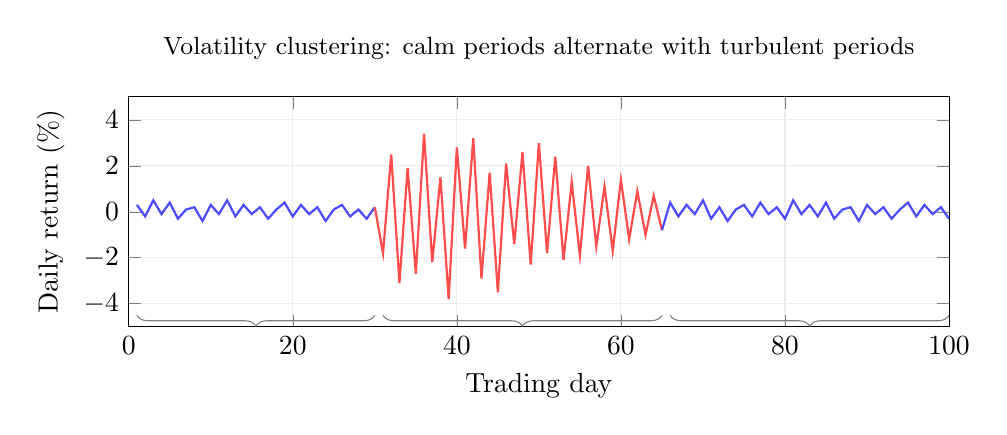
\begin{tikzpicture}
\begin{axis}[
    width=12cm, height=4.5cm,
    xlabel={Trading day},
    ylabel={Daily return (\%)},
    xmin=0, xmax=100,
    ymin=-5, ymax=5,
    grid=major,
    grid style={gray!15},
    ytick={-4,-2,0,2,4},
    xtick={0,20,40,60,80,100},
    every axis plot/.append style={mark=none},
    title={\small Volatility clustering: calm periods alternate with turbulent periods},
    title style={at={(0.5,1.05)}},
  ]

  % Calm period (days 1-30): small returns
  \addplot[blue!70, thick] coordinates {
    (1,0.3) (2,-0.2) (3,0.5) (4,-0.1) (5,0.4) (6,-0.3) (7,0.1)
    (8,0.2) (9,-0.4) (10,0.3) (11,-0.1) (12,0.5) (13,-0.2) (14,0.3)
    (15,-0.1) (16,0.2) (17,-0.3) (18,0.1) (19,0.4) (20,-0.2)
    (21,0.3) (22,-0.1) (23,0.2) (24,-0.4) (25,0.1) (26,0.3)
    (27,-0.2) (28,0.1) (29,-0.3) (30,0.2)
  };

  % Turbulent period (days 31-65): large returns
  \addplot[red!70, thick] coordinates {
    (30,0.2) (31,-1.8) (32,2.5) (33,-3.1) (34,1.9) (35,-2.7)
    (36,3.4) (37,-2.2) (38,1.5) (39,-3.8) (40,2.8) (41,-1.6)
    (42,3.2) (43,-2.9) (44,1.7) (45,-3.5) (46,2.1) (47,-1.4)
    (48,2.6) (49,-2.3) (50,3.0) (51,-1.8) (52,2.4) (53,-2.1)
    (54,1.3) (55,-1.9) (56,2.0) (57,-1.5) (58,1.1) (59,-1.7)
    (60,1.4) (61,-1.2) (62,0.9) (63,-1.0) (64,0.7) (65,-0.8)
  };

  % Calm again (days 65-100)
  \addplot[blue!70, thick] coordinates {
    (65,-0.8) (66,0.4) (67,-0.2) (68,0.3) (69,-0.1) (70,0.5)
    (71,-0.3) (72,0.2) (73,-0.4) (74,0.1) (75,0.3) (76,-0.2)
    (77,0.4) (78,-0.1) (79,0.2) (80,-0.3) (81,0.5) (82,-0.1)
    (83,0.3) (84,-0.2) (85,0.4) (86,-0.3) (87,0.1) (88,0.2)
    (89,-0.4) (90,0.3) (91,-0.1) (92,0.2) (93,-0.3) (94,0.1)
    (95,0.4) (96,-0.2) (97,0.3) (98,-0.1) (99,0.2) (100,-0.3)
  };

  % Annotations
  \draw[decorate, decoration={brace, amplitude=4pt, mirror}, gray]
    (axis cs:1,-4.5) -- (axis cs:30,-4.5)
    node[midway, below=5pt, font=\footnotesize, gray] {calm};
  \draw[decorate, decoration={brace, amplitude=4pt, mirror}, gray]
    (axis cs:31,-4.5) -- (axis cs:65,-4.5)
    node[midway, below=5pt, font=\footnotesize, gray] {turbulent};
  \draw[decorate, decoration={brace, amplitude=4pt, mirror}, gray]
    (axis cs:66,-4.5) -- (axis cs:100,-4.5)
    node[midway, below=5pt, font=\footnotesize, gray] {calm};

\end{axis}
\end{tikzpicture}
\end{center}

\citet{Engle1982} proposed the ARCH($q$) model. In its simplest form, ARCH(1):
%
\begin{equation}
\label{eq:arch1}
\sigma^2_t = \omega + \alpha_1 \, r^2_{t-1}
\end{equation}
%
\begin{itemize}[nosep]
  \item $\sigma^2_t$: conditional variance for period $t$ (the quantity we forecast)
  \item $\omega > 0$: baseline variance level, ensuring $\sigma^2_t$ stays positive
        even when $r_{t-1} = 0$
  \item $\alpha_1 \geq 0$: sensitivity to the most recent squared return
  \item $r^2_{t-1}$: squared return from the previous period, a noisy proxy for
        realized variance
\end{itemize}

The general ARCH($q$) model adds more lags:
%
\begin{equation}
\label{eq:archq}
\sigma^2_t = \omega + \sum_{i=1}^{q} \alpha_i \, r^2_{t-i}
\end{equation}
%
\begin{itemize}[nosep]
  \item $q$: number of lags included
  \item $\alpha_i \geq 0$: weight on the squared return from $i$ days ago
\end{itemize}

\begin{warning}[ARCH's Parameter Problem]
Volatility is persistent: a shock today still affects volatility weeks later.
Capturing this with ARCH requires many lags ($q = 10$ or more), each with its own
parameter. This makes estimation fragile and overfitting likely. GARCH solves this.
\end{warning}


%% ═══════════════════════════════════════════════════════════════
\section{GARCH(1,1): The Workhorse Model}
\label{sec:garch11}
%% ═══════════════════════════════════════════════════════════════

ARCH needs many parameters to capture persistence. The key insight of GARCH is
to add a single feedback term: let yesterday's \emph{conditional variance} help
predict today's.

\begin{intuition}[GARCH as Exponential Smoothing]
Think of a weather forecast. Tomorrow's temperature forecast depends on two things:
(1) what actually happened today (the ``news''), and (2) what you predicted
yesterday. GARCH works the same way: the new volatility forecast blends today's
squared return (news) with yesterday's forecast (memory). A single memory term
replaces an infinite history of squared returns.
\end{intuition}

Today's variance forecast feeds into tomorrow's, creating a self-reinforcing loop
that captures persistence (see diagram).

\begin{center}
\begin{tikzpicture}[
    node distance=2.2cm and 3.0cm,
    every node/.style={font=\small}
  ]
  % Nodes
  \node[flowblock, fill=blue!10, minimum width=2.5cm]
    (sig2prev) {$\sigma^2_{t-1}$\\(yesterday's\\forecast)};
  \node[flowblock, fill=orange!10, minimum width=2.5cm, right=3.5cm of sig2prev]
    (r2prev) {$r^2_{t-1}$\\(yesterday's\\squared return)};
  \node[flowblock, fill=green!10, minimum width=2.8cm,
        below right=2.0cm and 0.25cm of sig2prev]
    (sig2t) {$\sigma^2_{t}$\\(today's forecast)};
  \node[flowblock, fill=green!10, minimum width=2.8cm, below=2.0cm of sig2t]
    (sig2next) {$\sigma^2_{t+1}$\\(tomorrow's forecast)};
  \node[flowblock, fill=orange!10, minimum width=2.5cm,
        right=2.5cm of sig2t]
    (r2t) {$r^2_{t}$\\(today's\\squared return)};

  % Arrows
  \draw[arrow] (sig2prev) -- node[left, pos=0.4] {$\beta$} (sig2t);
  \draw[arrow] (r2prev) -- node[right, pos=0.4] {$\alpha$} (sig2t);
  \draw[arrow] (sig2t) -- node[left, pos=0.4] {$\beta$} (sig2next);
  \draw[arrow] (r2t) -- node[right, pos=0.4] {$\alpha$} (sig2next);

  % Omega
  \node[left=0.6cm of sig2t, text=gray] (omega1) {$+\;\omega$};
  \node[left=0.6cm of sig2next, text=gray] (omega2) {$+\;\omega$};

  % Feedback label
  \draw[dashed, gray, thick, rounded corners]
    (sig2t.south west) -- ($(sig2t.south west)+(-1.8,0)$)
    -- ($(sig2t.south west |- sig2next.north west)+(-1.8,0)$)
    -- (sig2next.north west);
  \node[gray, font=\footnotesize, anchor=east]
    at ($(sig2t.south west |- sig2next.north)+(-1.9,0.30)$)
    {feedback loop};
\end{tikzpicture}
\end{center}

\citet{bollerslev1986} introduced the GARCH(1,1) model:
%
\begin{equation}
\label{eq:garch11}
\sigma^2_t = \omega + \alpha \, r^2_{t-1} + \beta \, \sigma^2_{t-1}
\end{equation}
%
\begin{itemize}[nosep]
  \item $\sigma^2_t$: conditional variance for period $t$
  \item $\omega > 0$: intercept, related to the long-run average variance
  \item $\alpha \geq 0$: reaction coefficient; how strongly the model reacts to
        new information (yesterday's squared return)
  \item $\beta \geq 0$: persistence coefficient; how much of yesterday's variance
        forecast carries forward
  \item $r^2_{t-1}$: yesterday's squared return (the ``shock'' or ``news'')
  \item $\sigma^2_{t-1}$: yesterday's conditional variance forecast (the ``memory'')
\end{itemize}

\begin{projectconnection}[Why This Matters]
GARCH(1,1) is your simplest conditional-variance baseline. In a model horse race,
any ML model or HAR variant that cannot beat GARCH(1,1) out of sample is not worth
the added complexity. Typical $\alpha + \beta \approx 0.98$ for equity indices,
meaning volatility shocks are extremely persistent, the same stylized fact that HAR
captures with its weekly and monthly RV components.
\end{projectconnection}

\begin{definition}[Stationarity Condition for GARCH(1,1)]
\label{def:garch-stationarity}
The process is covariance-stationary if and only if
$\alpha + \beta < 1$. When this holds, the unconditional (long-run) variance is:
%
\begin{equation}
\label{eq:garch-uncond}
\bar{\sigma}^2 = \frac{\omega}{1 - \alpha - \beta}
\end{equation}
%
\begin{itemize}[nosep]
  \item $\bar{\sigma}^2$: the unconditional variance, i.e., the level to which
        $\sigma^2_t$ mean-reverts over time
  \item $\alpha + \beta$: total persistence; values close to 1 mean slow
        mean-reversion (volatility shocks are long-lived)
\end{itemize}
If $\alpha + \beta = 1$, the model becomes IGARCH (Integrated GARCH): shocks
never decay, and the unconditional variance is undefined
\citep{engle1986}.
\end{definition}

\begin{intuition}[In Plain English]
The unconditional variance is the ``gravity'' level that the conditional variance
always pulls toward. This is mean reversion in volatility, and the speed of that
reversion is $1 - \alpha - \beta$.
\end{intuition}

\begin{projectconnection}[Why This Matters]
When you forecast RV at the 22-day horizon, mean-reversion speed matters enormously.
A GARCH model with $\alpha + \beta = 0.98$ will still forecast elevated volatility
three weeks after a shock, while HAR's monthly component captures the same
persistence more flexibly. Comparing the implied half-lives of GARCH versus HAR
forecasts is a simple diagnostic for your project.
\end{projectconnection}

\begin{workedexample}{GARCH(1,1) One-Step Forecast}
\label{ex:garch11-calc}
Suppose you have estimated parameters $\omega = 0.00001$, $\alpha = 0.08$,
$\beta = 0.90$. Yesterday's return was $r_{t-1} = -0.03$ (a 3\% loss), and
yesterday's conditional variance was $\sigma^2_{t-1} = 0.0004$
(implying $\sigma_{t-1} = 0.02$, or 2\% daily vol).

\textbf{Step 1: Compute the forecast.}
Summing the baseline, news, and memory components gives
$\sigma^2_t = 0.00001 + 0.000072 + 0.00036 = 0.000442$, so
$\sigma_t = \sqrt{0.000442} \approx 2.10\%$.

Most of the forecast (81\%) comes from the
memory term $\beta \sigma^2_{t-1}$, reflecting the high persistence typical of
financial volatility.

\textbf{Step 2: Check long-run variance.}
%
\[
\bar{\sigma}^2 = \frac{0.00001}{1 - 0.08 - 0.90}
  = \frac{0.00001}{0.02} = 0.0005
\quad\Rightarrow\quad
\bar{\sigma} \approx 2.24\%
\]

With $\alpha + \beta = 0.98$, mean-reversion is very slow: it takes roughly
$\ln(0.5)/\ln(0.98) \approx 34$ days for the conditional variance to close half
the gap to $\bar{\sigma}^2$.
\end{workedexample}

\begin{keyidea}[GARCH(1,1) Is Usually Enough]
\label{idea:garch11-enough}
\citet{hansen2005forecast} compared 330 GARCH-type models on exchange rate and
equity data. For exchange rates, no model significantly outperformed GARCH(1,1). For
equities, models with a leverage effect (Section~\ref{sec:leverage}) did better, but
higher-order specifications like GARCH(2,1) or GARCH(1,2) provided negligible
improvement. In practice, GARCH(1,1) captures the bulk of conditional variance
dynamics. The gains from asymmetric extensions come from modeling leverage, not from
adding lags.
\end{keyidea}


%% ═══════════════════════════════════════════════════════════════
\section{The Leverage Effect}
\label{sec:leverage}
%% ═══════════════════════════════════════════════════════════════

GARCH(1,1) treats positive and negative returns symmetrically: a $+3\%$ return and
a $-3\%$ return produce the same $r^2_{t-1} = 0.0009$ and thus the same volatility
forecast. In real equity markets, this is wrong.

\begin{intuition}[Why Negative Returns Increase Volatility More]
\citet{Black1976} documented this asymmetry and proposed an explanation. When a
stock drops, the firm's equity value falls while its debt stays fixed. The firm
becomes more leveraged (higher debt-to-equity ratio), making its equity riskier, so
volatility rises. A positive return has the opposite effect but to a smaller degree.
This ``leverage effect'' is one of the most robust stylized facts in equity markets.
\end{intuition}

For the same magnitude of return, negative returns produce a larger volatility
response than positive returns (diagram).

\begin{center}
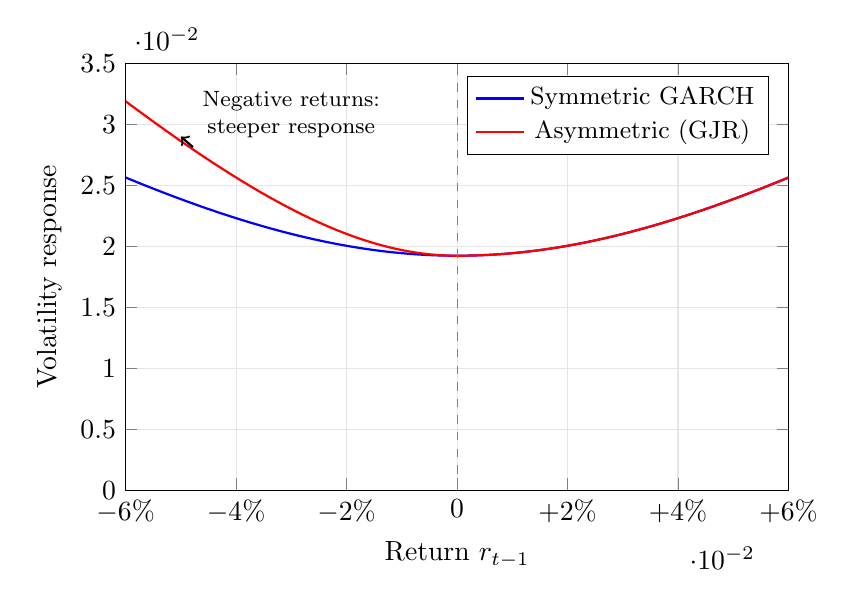
\begin{tikzpicture}
\begin{axis}[
    width=10cm, height=7cm,
    xlabel={Return $r_{t-1}$},
    ylabel={Volatility response},
    xmin=-0.06, xmax=0.06,
    ymin=0, ymax=0.035,
    grid=major,
    grid style={gray!20},
    legend pos=north east,
    legend style={font=\small},
    xtick={-0.06,-0.04,-0.02,0,0.02,0.04,0.06},
    xticklabels={$-6\%$,$-4\%$,$-2\%$,$0$,$+2\%$,$+4\%$,$+6\%$},
    ytick={0,0.005,0.01,0.015,0.02,0.025,0.03,0.035},
  ]

  % Symmetric GARCH: alpha * r^2 with alpha = 0.08, scale to vol
  \addplot[blue, thick, domain=-0.06:0.06, samples=100]
    {sqrt(0.00001 + 0.08*x^2 + 0.90*0.0004)};
  \addlegendentry{Symmetric GARCH}

  % Asymmetric (GJR-like): extra gamma for negative returns
  \addplot[red, thick, domain=-0.06:0, samples=50]
    {sqrt(0.00001 + (0.08 + 0.10)*x^2 + 0.90*0.0004)};
  \addplot[red, thick, domain=0:0.06, samples=50, forget plot]
    {sqrt(0.00001 + 0.08*x^2 + 0.90*0.0004)};
  \addlegendentry{Asymmetric (GJR)}

  % Vertical line at zero
  \draw[dashed, gray] (axis cs:0,0) -- (axis cs:0,0.035);

  % Annotations
  \node[font=\footnotesize, align=center, anchor=north] (negann) at (axis cs:-0.030, 0.0335) {Negative returns:\\steeper response};
  \draw[->, thick] (negann.south west) -- (axis cs:-0.050, 0.0290);

\end{axis}
\end{tikzpicture}
\end{center}

Standard GARCH(1,1) cannot capture this asymmetry because it depends on $r^2_{t-1}$,
which discards the sign of the return. The next two sections present models that fix
this.


%% ═══════════════════════════════════════════════════════════════
\section{GJR-GARCH: A Simple Asymmetric Extension}
\label{sec:gjr}
%% ═══════════════════════════════════════════════════════════════

The most direct way to capture leverage is to add an indicator function that
activates only for negative returns.

\citet{gjr1993} proposed:
%
\begin{equation}
\label{eq:gjr}
\sigma^2_t = \omega + \alpha \, r^2_{t-1}
  + \gamma \, \mathbf{1}_{\{r_{t-1} < 0\}} \, r^2_{t-1}
  + \beta \, \sigma^2_{t-1}
\end{equation}
%
\begin{itemize}[nosep]
  \item $\omega, \alpha, \beta$: same roles as in GARCH(1,1)
        (Equation~\ref{eq:garch11})
  \item $\gamma \geq 0$: the asymmetry (leverage) parameter
  \item $\mathbf{1}_{\{r_{t-1} < 0\}}$: indicator function equal to 1 when
        $r_{t-1} < 0$, and 0 otherwise
\end{itemize}

The effect is straightforward:
\begin{itemize}[nosep]
  \item After a \emph{positive} return: the effective coefficient on $r^2_{t-1}$ is
        just $\alpha$.
  \item After a \emph{negative} return: the effective coefficient is
        $\alpha + \gamma$, giving a stronger volatility response.
\end{itemize}

\begin{projectconnection}[Why This Matters]
The leverage effect is one of the strongest predictable patterns in equity volatility.
Adding an asymmetry term (whether in GJR-GARCH or as a signed-return feature in your
ML model) typically improves QLIKE by 5--15\%. If your HAR baseline does not include
a negative-return indicator, GJR-GARCH shows exactly why it should.
\end{projectconnection}

%% ═══════════════════════════════════════════════════════════════
\section{EGARCH: Log-Variance and Guaranteed Positivity}
\label{sec:egarch}
%% ═══════════════════════════════════════════════════════════════

GJR-GARCH has a practical annoyance: you need parameter constraints
($\omega > 0$, $\alpha \geq 0$, $\alpha + \gamma \geq 0$, $\beta \geq 0$) to
ensure $\sigma^2_t > 0$. Unconstrained optimization sometimes produces estimates
that violate these bounds.

\citet{nelson1991} proposed EGARCH, which models the \emph{log} of variance. Since
$\exp(\cdot)$ is always positive, the variance is automatically positive regardless
of parameter signs.

\begin{equation}
\label{eq:egarch}
\ln \sigma^2_t
  = \omega
  + \beta \ln \sigma^2_{t-1}
  + \alpha \left( \frac{|r_{t-1}|}{\sigma_{t-1}} - \sqrt{\frac{2}{\pi}} \right)
  + \gamma \, \frac{r_{t-1}}{\sigma_{t-1}}
\end{equation}
%
\begin{itemize}[nosep]
  \item $\ln \sigma^2_t$: log conditional variance (the model's target)
  \item $\omega$: intercept on the log-variance scale (can be any real number)
  \item $\beta$: persistence of log-variance; $|\beta| < 1$ for stationarity
  \item $|r_{t-1}|/\sigma_{t-1}$: the absolute value of the standardized return,
        measuring shock magnitude
  \item $\sqrt{2/\pi}$: the expected value of $|z|$ when $z \sim \N(0,1)$;
        subtracting it centers the magnitude term at zero
  \item $\alpha$: the size effect; controls how strongly large shocks (of either
        sign) increase variance
  \item $r_{t-1}/\sigma_{t-1}$: the signed standardized return
  \item $\gamma$: the sign effect (asymmetry parameter); $\gamma < 0$ means
        negative returns increase log-variance
\end{itemize}

\begin{intuition}[How the Sign Effect Works]
The $\gamma$ term adds $\gamma \cdot z_{t-1}$ to log-variance, where
$z_{t-1} = r_{t-1}/\sigma_{t-1}$ is the standardized return. If $\gamma = -0.10$
and the standardized return is $z = -2$ (a two-standard-deviation loss), the
contribution is $(-0.10)(-2) = +0.20$: log-variance rises. If $z = +2$ (a
two-standard-deviation gain), the contribution is $(-0.10)(+2) = -0.20$:
log-variance falls. The same shock magnitude produces opposite effects depending on
sign.
\end{intuition}

\begin{projectconnection}[Why This Matters]
Many ML models for realized volatility also work in log space ($\log \RV_t$), just as
EGARCH does. If you include EGARCH as a baseline, its sign-effect coefficient $\gamma$
gives you a direct comparison point for how well your ML model captures asymmetry.
\end{projectconnection}

\begin{warning}[EGARCH Forecasting Complication]
Multi-step forecasts from EGARCH require computing $\E[\exp(\cdot)]$, which does
not simplify as cleanly as for linear GARCH. In practice, simulation-based forecasts
are used for horizons beyond one step.
\end{warning}


%% ═══════════════════════════════════════════════════════════════
\section{Long Memory in Volatility: FIGARCH}
\label{sec:figarch}
%% ═══════════════════════════════════════════════════════════════

Volatility autocorrelations in financial data decay very slowly. If you compute the
autocorrelation of daily squared returns (or absolute returns) at lags 1, 5, 20,
100, you find that the autocorrelation is still positive even at lag 100. Standard
GARCH(1,1) implies \emph{exponential} decay of autocorrelations, which is too fast.

\begin{prereq}[Long Memory and Fractional Integration]
A time series has \emph{long memory} if its autocorrelations decay at a hyperbolic
(power-law) rate rather than an exponential rate. In the context of ARIMA, a
non-integer differencing parameter $d \in (0, 0.5)$ produces this behavior: the
series is neither stationary ($d = 0$) nor unit-root ($d = 1$), but something in
between. The same idea can be applied to the variance equation of a GARCH model.
\end{prereq}

\citet{baillie1996} introduced FIGARCH, which replaces the integer-differencing
implicit in GARCH with fractional differencing.

\begin{definition}[FIGARCH Differencing Parameter]
\label{def:figarch-d}
The FIGARCH model introduces a parameter $d \in (0, 1)$ governing the rate at which
past shocks influence current variance:
%
\begin{itemize}[nosep]
  \item $d = 0$: equivalent to GARCH; shock impact decays exponentially (short
        memory)
  \item $d = 1$: equivalent to IGARCH; shock impact never decays (unit root in
        variance)
  \item $0 < d < 1$: shock impact decays hyperbolically (long memory); past shocks
        matter, but their influence eventually fades
\end{itemize}
\end{definition}

The full FIGARCH(1,$d$,1) specification is written using the lag operator $L$:
%
\begin{equation}
\label{eq:figarch}
(1 - \beta L)\sigma^2_t
  = \omega + \bigl[1 - \beta L - (1 - \phi L)(1 - L)^d\bigr] r^2_t
\end{equation}
%
\begin{itemize}[nosep]
  \item $L$: lag operator ($L \, x_t = x_{t-1}$)
  \item $(1-L)^d$: fractional differencing operator with parameter $d$
  \item $\phi$: an additional ARCH-side parameter
  \item $\beta$: persistence parameter, same role as in GARCH
\end{itemize}

The key point is not the algebra but the implication: FIGARCH matches the slow decay
of volatility autocorrelations far better than GARCH.

\begin{projectconnection}[Why This Matters]
Long memory in volatility is precisely why HAR works: its weekly and monthly
components act as a discrete approximation to the slow-decaying memory that FIGARCH
models continuously. If your ML residual model finds that long-lag features improve
forecasts, FIGARCH's $d$ parameter gives you a theoretical explanation for why.
\end{projectconnection}

\begin{keyidea}[FIGARCH vs.\ Rough Volatility]
Both FIGARCH and rough volatility models (Chapter~\ref{ch:rough}) address the same
empirical fact: volatility has long memory. FIGARCH does so within the discrete-time
GARCH framework by adding the parameter $d$. Rough volatility uses continuous-time
fractional Brownian motion with Hurst parameter $H \approx 0.1$. The two approaches
are complementary views of the same phenomenon.
\end{keyidea}


%% ═══════════════════════════════════════════════════════════════
\section{Realized GARCH: Bringing Intraday Data into GARCH}
\label{sec:realized-garch}
%% ═══════════════════════════════════════════════════════════════

Standard GARCH uses only daily returns to infer volatility. But if you have access
to intraday data, you can compute realized volatility ($\RV_t$, as defined in
Chapter~\ref{ch:rv}), a far more precise measure of what actually happened. Realized
GARCH incorporates $\RV_t$ directly into the GARCH framework.

\begin{intuition}[The Measurement Problem]
In GARCH, the conditional variance $\sigma^2_t$ is a latent (unobserved) variable.
The model infers it from the noisy signal $r^2_t$ (the squared daily return). But
$r^2_t$ is an extremely noisy estimator of daily variance: on average, the
noise-to-signal ratio exceeds 5. Realized volatility $\RV_t$ is computed from many
intraday returns and is orders of magnitude more precise. Realized GARCH exploits
this better signal.
\end{intuition}

The key addition in Realized GARCH is the measurement equation linking $\RV_t$ to the
latent conditional variance $h_t$ (see diagram).

\begin{center}
\begin{tikzpicture}[
    node distance=1.8cm and 2.5cm,
    every node/.style={font=\small}
  ]

  % Standard GARCH (left)
  \node[font=\bfseries] (title1) {Standard GARCH};
  \node[flowblock, fill=blue!10, below=0.8cm of title1, minimum width=2.2cm]
    (g_ht) {$h_t$};
  \node[flowblock, fill=orange!10, right=1.5cm of g_ht, minimum width=2.2cm]
    (g_r2) {$r^2_t$};
  \node[flowblock, fill=blue!10, below=1.5cm of g_ht, minimum width=2.2cm]
    (g_ht1) {$h_{t+1}$};

  \draw[arrow] (g_ht) -- node[left] {$\beta$} (g_ht1);
  \draw[arrow] (g_r2) -- node[right, pos=0.3] {$\alpha$} (g_ht1);

  % Realized GARCH (right)
  \node[font=\bfseries, right=5.5cm of title1] (title2) {Realized GARCH};
  \node[flowblock, fill=blue!10, below=0.8cm of title2, minimum width=2.2cm]
    (rg_ht) {$h_t$};
  \node[flowblock, fill=green!10, right=1.5cm of rg_ht, minimum width=2.2cm]
    (rg_rv) {$\RV_t$};
  \node[flowblock, fill=blue!10, below=1.5cm of rg_ht, minimum width=2.2cm]
    (rg_ht1) {$h_{t+1}$};

  % Measurement equation arrow
  \draw[arrow, dashed, intgreen] (rg_ht) -- node[above, font=\footnotesize]
    {measurement eq.} (rg_rv);

  % GARCH equation arrows
  \draw[arrow] (rg_ht) -- node[left] {$\beta$} (rg_ht1);
  \draw[arrow, intgreen, thick] (rg_rv) -- node[right, pos=0.3]
    {$\gamma$} (rg_ht1);

  % Dividing line
  \draw[gray, dashed] ([xshift=2.0cm]title1.east) ++(0,0.3)
    -- ++(0,-5.5);

\end{tikzpicture}
\end{center}

\citet{hansen2012realized} specify three equations. The return equation
is standard:
%
\begin{equation}
\label{eq:rgarch-return}
r_t = \sqrt{h_t}\; z_t, \qquad z_t \sim \N(0,1)
\end{equation}
%
\begin{itemize}[nosep]
  \item $r_t$: daily return
  \item $h_t$: conditional variance (the latent variable we model)
  \item $z_t$: standardized innovation, assumed i.i.d.\ standard normal
\end{itemize}

This is the standard return-generating process: the daily return is volatility times
a random shock. It is shared with standard GARCH and is not where Realized GARCH
innovates.

The measurement equation links the observed $\RV_t$ to the latent $h_t$:
%
\begin{equation}
\label{eq:rgarch-measurement}
\log \RV_t = \xi + \delta \log h_t + \tau(z_t) + u_t
\end{equation}
%
\begin{itemize}[nosep]
  \item $\log \RV_t$: log realized volatility (observed from intraday data)
  \item $\xi$: intercept allowing for a level difference between $\RV_t$ and $h_t$
  \item $\delta$: loading of $\log h_t$ on $\log \RV_t$; typically close to 1
  \item $\tau(z_t)$: a leverage function of the standardized return, capturing the
        asymmetry between positive and negative returns (often specified as
        $\tau_1 z_t + \tau_2(z_t^2 - 1)$)
  \item $u_t$: measurement noise, independent of $z_t$
\end{itemize}

The GARCH equation uses $\RV_t$ instead of $r^2_t$:
%
\begin{equation}
\label{eq:rgarch-garch}
\log h_{t+1} = \omega + \beta \log h_t + \gamma \log \RV_t
\end{equation}
%
\begin{itemize}[nosep]
  \item $\omega$: intercept on the log-variance scale
  \item $\beta$: persistence of the conditional variance
  \item $\gamma$: sensitivity to the realized measure; this is where intraday
        information enters the model
\end{itemize}

\begin{intuition}[In Plain English]
Realized GARCH is a three-part system. (1) Returns are driven by latent variance, as
usual. (2) The measurement equation says ``realized volatility is a noisy, possibly
biased reading of that latent variance, with an asymmetry correction.'' (3) The
GARCH equation says ``tomorrow's latent variance depends on today's latent variance
(persistence) plus today's realized volatility (new information).'' The key upgrade
over standard GARCH is in step (3): instead of feeding in the noisy squared return
$r^2_t$, you feed in $\RV_t$, which is orders of magnitude more precise.
\end{intuition}

\begin{projectconnection}[Why This Matters]
Realized GARCH is the bridge between the GARCH world and the RV world your project
lives in. It uses $\RV_t$ directly as an input, just as your HAR and ML models do.
Including Realized GARCH as a baseline lets you ask: ``Does my ML model add value
beyond what a well-specified parametric model can extract from the same $\RV_t$
data?'' If your ML model only matches Realized GARCH, the complexity may not be
justified.
\end{projectconnection}

\begin{keyresult}[Realized GARCH Outperforms Standard GARCH]
\citet{hansen2012realized} find that Realized GARCH with log-linear specification
substantially outperforms standard GARCH(1,1) in both in-sample fit and
out-of-sample forecasting on Dow Jones Industrial Average stocks. Squared returns
become statistically insignificant once a realized measure is included. The leverage
function $\tau(z_t)$ is highly significant, confirming the importance of asymmetry.
\end{keyresult}


%% ═══════════════════════════════════════════════════════════════
\section{The HEAVY Model}
\label{sec:heavy}
%% ═══════════════════════════════════════════════════════════════

Realized GARCH is not the only way to combine daily and intraday information.
\citet{shephard2010heavy} proposed the HEAVY (High-frEquency-bAsed VolatilitY)
model, which takes a different but related approach: instead of treating $\RV_t$ as
a noisy measurement of a latent $h_t$, HEAVY models both the conditional variance of
returns and the conditional expectation of $\RV_t$ as a joint system.

The HEAVY system has two equations. The first governs the conditional variance of
daily returns:
%
\begin{equation}
\label{eq:heavy-return}
\sigma^2_{R,t} = \omega_R + \alpha_R \, \RV_{t-1} + \beta_R \, \sigma^2_{R,t-1}
\end{equation}
%
\begin{itemize}[nosep]
  \item $\sigma^2_{R,t}$: conditional variance of daily returns
  \item $\RV_{t-1}$: yesterday's realized variance (replaces $r^2_{t-1}$ from GARCH)
  \item $\alpha_R$: sensitivity to the realized measure
  \item $\beta_R$: persistence of the return variance
\end{itemize}

The second governs the conditional expectation of realized variance:
%
\begin{equation}
\label{eq:heavy-rv}
\mu_{M,t} = \omega_M + \alpha_M \, \RV_{t-1} + \beta_M \, \mu_{M,t-1}
\end{equation}
%
\begin{itemize}[nosep]
  \item $\mu_{M,t}$: conditional expectation of $\RV_t$ (what you expect today's
        realized variance to be)
  \item $\alpha_M, \beta_M$: analogous to GARCH parameters but for the realized
        measure
\end{itemize}

\begin{intuition}[In Plain English]
HEAVY runs two GARCH-like equations side by side. The first forecasts the variance of
daily returns, and the second forecasts realized variance itself. Both use
yesterday's $\RV$ as input instead of $r^2$. Think of it as two parallel trackers:
one for ``what will the daily return variance be?'' and one for ``what will intraday
volatility look like?''
\end{intuition}

\begin{projectconnection}[Why This Matters]
The second HEAVY equation (Equation~\ref{eq:heavy-rv}) is essentially forecasting
$\RV_t$ using an AR(1) in $\RV$ with GARCH-style persistence, making it a
close relative of the HAR model's daily component. Comparing HEAVY's $\mu_{M,t}$
forecasts against your HAR forecasts at the one-day horizon reveals how much the
multi-horizon structure of HAR adds beyond a simple autoregressive specification.
\end{projectconnection}

\begin{keyresult}[HEAVY Model Performance]
\citet{shephard2010heavy} find that the HEAVY model outperforms GARCH both in-sample
and out-of-sample across a range of asset classes. Forecast gains are most pronounced
at short horizons (one to five days). The model adjusts quickly to structural breaks
in the volatility level because $\RV_{t-1}$ responds immediately to intraday price
variation, while GARCH must wait for the slow accumulation of squared daily returns.
\end{keyresult}


%% ═══════════════════════════════════════════════════════════════
\section{Comparison: GARCH vs.\ Realized GARCH vs.\ HEAVY}
\label{sec:comparison}
%% ═══════════════════════════════════════════════════════════════

The key distinction across the three approaches is the data input: standard GARCH
uses only daily returns, while Realized GARCH and HEAVY incorporate intraday
information through $\RV_t$ (see table).

\begin{center}
\renewcommand{\arraystretch}{1.3}
\begin{tabular}{@{} l p{3.2cm} p{3.2cm} p{3.2cm} @{}}
\toprule
& \textbf{GARCH(1,1)} & \textbf{Realized GARCH} & \textbf{HEAVY} \\
\midrule
\textbf{Data input}
  & Daily returns only
  & Daily returns $+$ $\RV_t$
  & Daily returns $+$ $\RV_t$ \\[2pt]
\textbf{Volatility driver}
  & $r^2_{t-1}$
  & $\log \RV_t$
  & $\RV_{t-1}$ \\[2pt]
\textbf{Latent variance}
  & Yes ($\sigma^2_t$)
  & Yes ($h_t$), linked to $\RV_t$ via measurement eq.
  & Two: $\sigma^2_{R,t}$ (returns) and $\mu_{M,t}$ (RV) \\[2pt]
\textbf{Leverage effect}
  & Not in basic form; needs GJR or EGARCH
  & Built in via $\tau(z_t)$
  & Not in basic form; extensions exist \\[2pt]
\textbf{Structural breaks}
  & Slow adjustment
  & Faster (uses $\RV_t$)
  & Fastest (direct $\RV$ input) \\[2pt]
\textbf{Estimation}
  & MLE on daily returns
  & Joint MLE
  & Equation-by-equation or joint MLE \\[2pt]
\textbf{Use when}
  & No intraday data available
  & Intraday data available; want a single integrated framework
  & Intraday data available; want fast response to regime changes \\
\bottomrule
\end{tabular}
\end{center}

\begin{warning}[GARCH Is Not a Straw Man]
When intraday data is unavailable (many asset classes, historical periods, or
emerging markets), GARCH remains the best option. Even with intraday data, GARCH
serves as a useful baseline: any more complex model should demonstrably outperform
it. \citet{andersen1998} showed that GARCH forecasts appear poor only when evaluated
against noisy proxies like $r^2_t$; evaluated against $\RV_t$, they perform
respectably.
\end{warning}


%% ═══════════════════════════════════════════════════════════════
\section{Summary}
\label{sec:garch-summary}
%% ═══════════════════════════════════════════════════════════════

\begin{itemize}[nosep]
  \item ARCH \citep{Engle1982} models conditional variance as a function of past
        squared returns but requires many lags to capture persistence.

  \item GARCH(1,1) \citep{bollerslev1986} adds a single feedback term
        ($\beta \sigma^2_{t-1}$), capturing persistence with just three parameters
        ($\omega, \alpha, \beta$).

  \item The stationarity condition is $\alpha + \beta < 1$; the unconditional
        variance is $\omega / (1 - \alpha - \beta)$.

  \item Higher-order GARCH($p,q$) rarely improves on GARCH(1,1) in practice
        \citep{hansen2005forecast}.

  \item The leverage effect \citep{Black1976}: negative returns increase volatility
        more than positive returns of the same magnitude.

  \item GJR-GARCH \citep{gjr1993} adds an indicator term
        $\gamma \, \mathbf{1}_{\{r<0\}} \, r^2_{t-1}$ to capture leverage simply.

  \item EGARCH \citep{nelson1991} models log-variance, guaranteeing positivity
        without parameter constraints and capturing both sign and size effects.

  \item FIGARCH \citep{baillie1996} introduces fractional integration ($d \in (0,1)$)
        to match the slow, hyperbolic decay of volatility autocorrelations.

  \item Realized GARCH \citep{hansen2012realized} links $\RV_t$ to the latent
        conditional variance via a measurement equation, substantially outperforming
        standard GARCH.

  \item The HEAVY model \citep{shephard2010heavy} builds a joint system for daily
        return variance and $\RV_t$, adjusting quickly to structural breaks.

  \item GARCH remains the right baseline when intraday data is unavailable.

  \item The HAR model (Chapter~\ref{ch:har}) offers a simpler, non-parametric
        alternative for RV forecasting that often matches or beats Realized GARCH.
\end{itemize}


%% ═══════════════════════════════════════════════════════════════
\section*{Key Results}
\label{sec:garch-key-results}
%% ═══════════════════════════════════════════════════════════════

\begin{center}
\renewcommand{\arraystretch}{1.3}
\begin{tabular}{@{} p{3.5cm} l p{6.5cm} @{}}
\toprule
\textbf{Result} & \textbf{Source} & \textbf{Finding} \\
\midrule
ARCH model
  & \citet{Engle1982}
  & Conditional variance depends on past squared returns;
    Nobel Prize--winning framework \\
GARCH(1,1)
  & \citet{bollerslev1986}
  & Single memory term replaces many ARCH lags;
    three parameters capture the bulk of variance dynamics \\
Leverage effect
  & \citet{Black1976}
  & Negative returns increase volatility more than positive
    returns of the same magnitude \\
GJR-GARCH
  & \citet{gjr1993}
  & Indicator-based asymmetry; effective coefficient on
    negative shocks is $\alpha + \gamma$ \\
EGARCH
  & \citet{nelson1991}
  & Log-variance specification; no positivity constraints;
    separates sign and size effects \\
GARCH(1,1) benchmark
  & \citet{hansen2005forecast}
  & Among 330 models, no significant improvement from
    higher-order lags; leverage matters for equities \\
FIGARCH
  & \citet{baillie1996}
  & Fractional integration parameter $d$ captures
    hyperbolic decay of volatility autocorrelations \\
Realized GARCH
  & \citet{hansen2012realized}
  & Incorporating $\RV_t$ via measurement equation
    substantially outperforms daily-return-only GARCH \\
HEAVY model
  & \citet{shephard2010heavy}
  & Joint return/RV system; fast adjustment to regime
    changes; strongest gains at short horizons \\
\bottomrule
\end{tabular}
\end{center}
